%!TEX program = xelatex
%将长宽比设为 16:9,帧尺寸设为 160mm×90mm。
\documentclass[hyperref={bookmarks=false},aspectratio=169]{beamer}
\usepackage[utf8]{inputenc}
\usepackage{ctex}
\usepackage{graphicx}


% ---------------  Define theme and color scheme  -----------------
\usetheme[sidebarleft]{Baiter}  % 3 options: minimal, sidebarleft, sidebarright

% ------------  Information on the title page  --------------------
\title[试用期工作总结]
{\bfseries{试用期工作总结及工作内容}}

\subtitle{summary of probation work}

\author[]{黑志强\inst{1} }

\institute
{
  \inst{1}
  天天向上网络智能 \quad WISDAYTECH\\
  heizhiqiangair@163.com
  \begin{figure}[ht!]
    \center{
\includegraphics[width=0.1\textwidth]{./figures/logo550.png}}
  \end{figure}
}

\date{12/08/2017}


\AtBeginSection[]
{
  \begin{frame}
    \frametitle{Table of Contents}
    \tableofcontents[currentsection]
  \end{frame}
}
%------------------------------------------------------------


\begin{document}

\frame{\titlepage}  % Creates title page

%---------   table of contents after title page  ------------
\begin{frame}
\frametitle{Table of Contents}
\tableofcontents
\end{frame}
%---------------------------------------------------------
%\usebackgroundtemplate{\includegraphics[width=\paperwidth,height=\paperheight]{./figures/dengta.jpg}}



\section{工作模块划分}


\begin{frame}
\frametitle{工作模块划分}

\begin{figure}[ht!]

\center{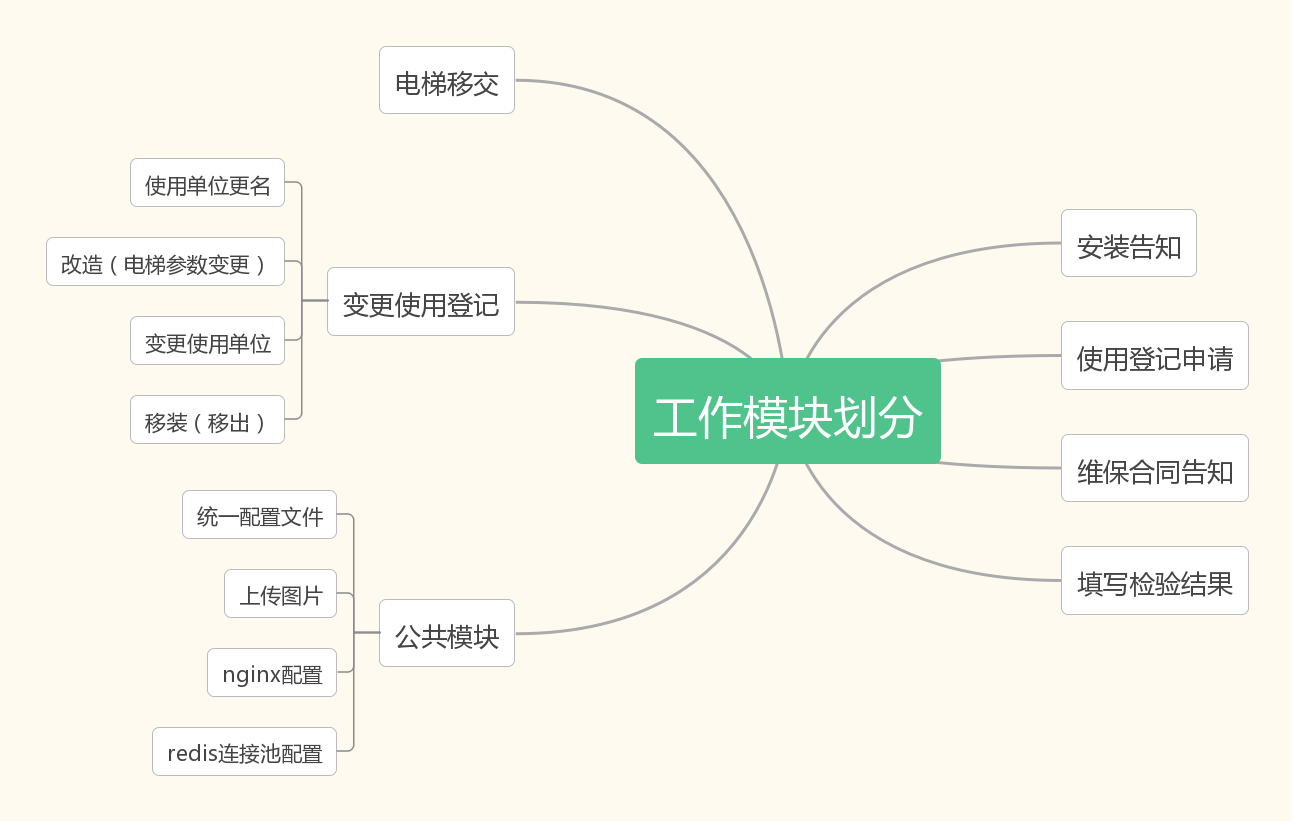
\includegraphics[width=0.8\textwidth]{./figures/summary1.png}}
\end{figure}

\end{frame}


\section{安装告知}


\begin{frame}
\frametitle{安装告知}

\begin{figure}[ht!]

\center{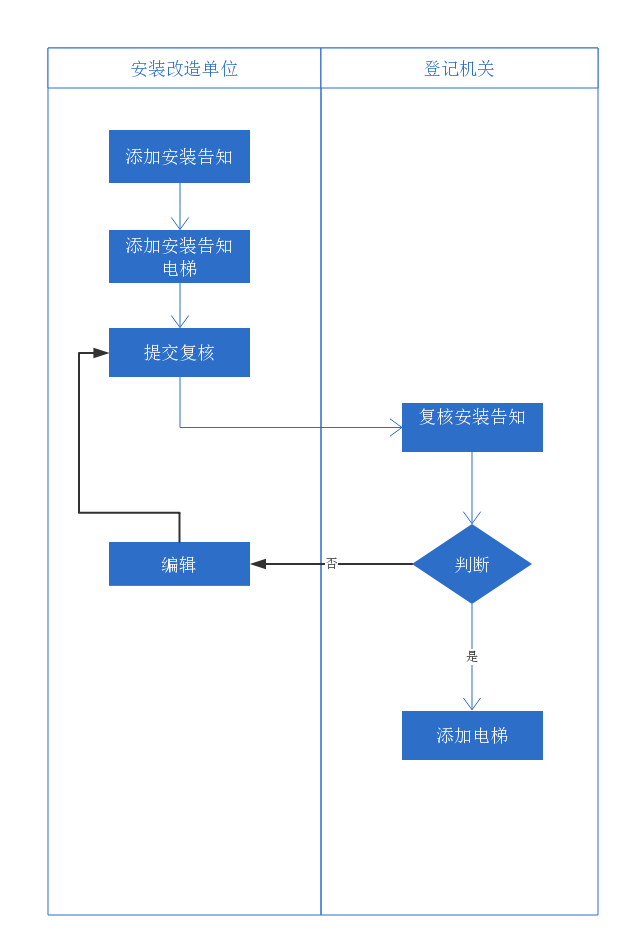
\includegraphics[width=0.4\textwidth]{./figures/instal-flow.png}}
\end{figure}

\end{frame}

\section{维保合同告知}


\begin{frame}
\frametitle{维保合同告知}

\begin{figure}[ht!]

\center{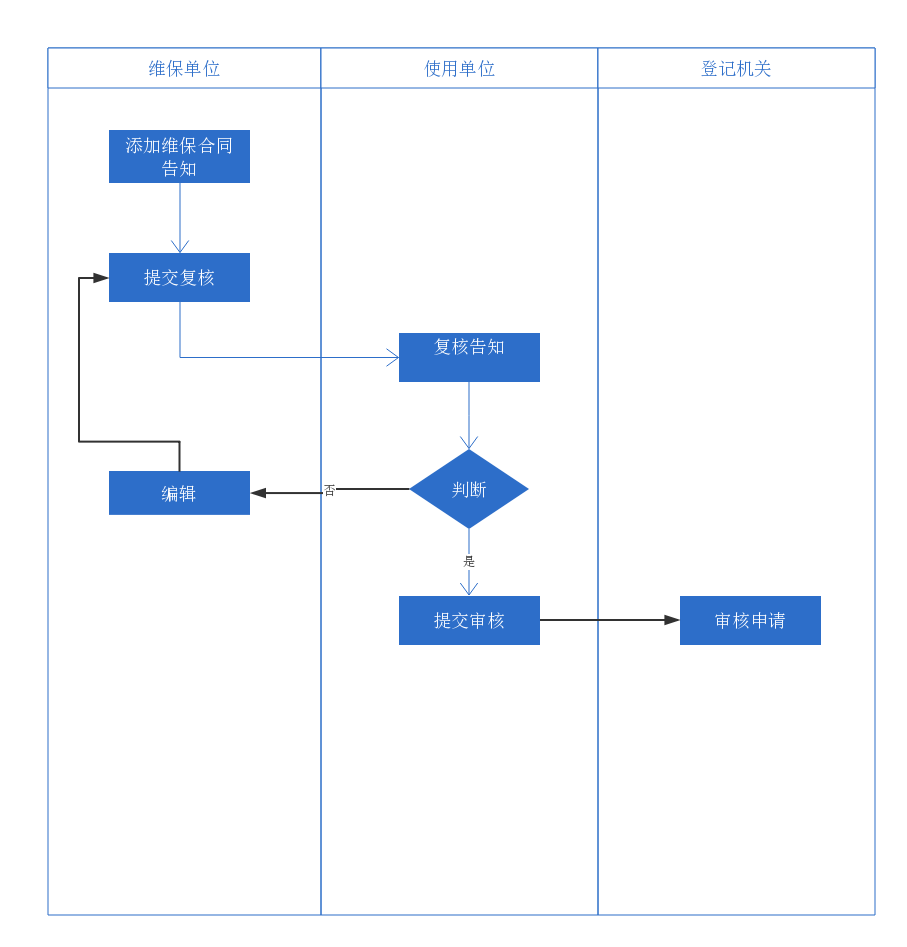
\includegraphics[width=0.6\textwidth]{./figures/maintain-flow.png}}
\end{figure}

\end{frame}

\section{使用登记申请}


\begin{frame}
\frametitle{使用登记申请}

\begin{figure}[ht!]

\center{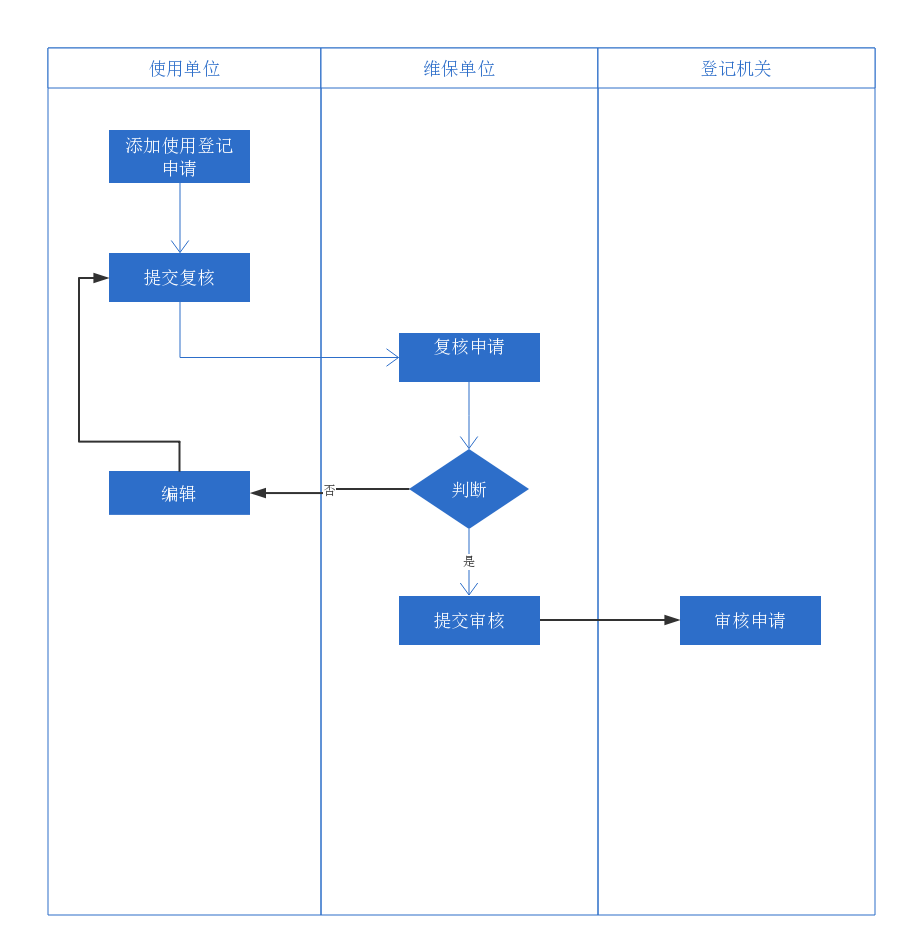
\includegraphics[width=0.6\textwidth]{./figures/useapply-flow.png}}
\end{figure}

\end{frame}

\section{变更使用登记}


\begin{frame}
\frametitle{变更使用登记}

\begin{figure}[ht!]

\center{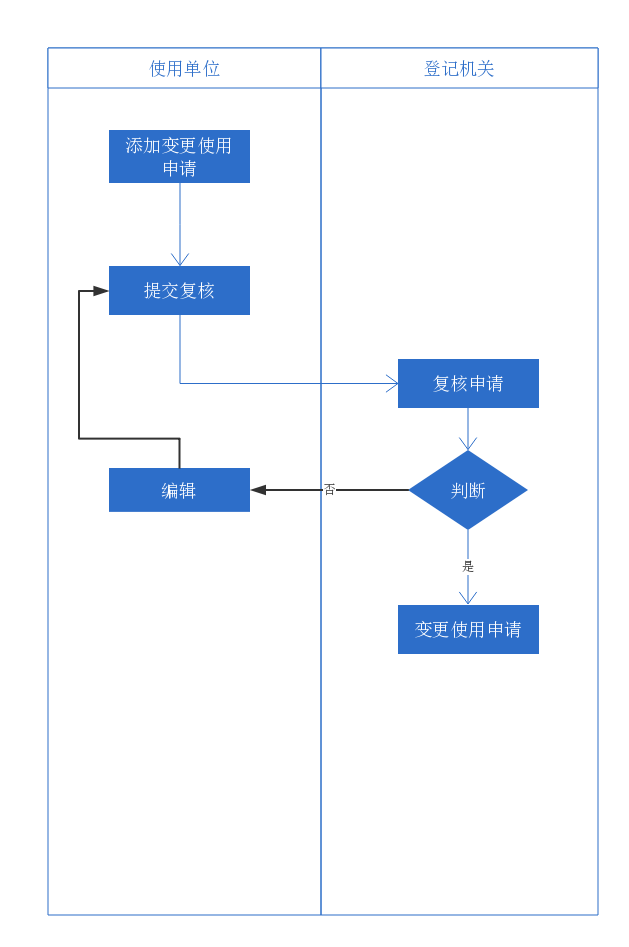
\includegraphics[width=0.4\textwidth]{./figures/alteruse-flow.png}}
\end{figure}

\end{frame}



\section{总结}

%---------------------------------------------------------
%Highlighting text
\begin{frame}
\frametitle{总结}

在此工作期间主要负责以下模块的开发工作

\begin{block}{模块}
安装告知;使用登记申请,变更使用登记(包含四个模块:使用单位更名,改造变更电梯参数,变更使用单位,移装|移出);填写检验结果;电梯移交;公共域部分模块。

\end{block}

在此工作期间遇到的问题
\begin{alertblock}{问题}
普元eos 在此期间掌握仍有不足,有些地方比较封闭,支持的类库比较老,不能很好的在这个基础上做扩展,比如:spring框架是2.*版本的,版本过低,大部分常用特性没有。
\end{alertblock}

\end{frame}



\section{扩展}

%---------------------------------------------------------
%Highlighting text
\begin{frame}
\frametitle{扩展}

可以扩展部分

\begin{block}{扩展}
在此抛开框架,针对java生态环境中,可以将文件存储改为目前较为流行的fastdfs,seaweedfs,支持分布式存储。

\end{block}


\end{frame}
%---------------------------------------------------------
%Two columns
\begin{frame}
\frametitle{August}

\begin{columns}[t]
\column{0.95\textwidth}
\begin{figure}
    \centering
    
\includegraphics[width=\columnwidth]{./figures/august-nocal.jpg}
    \caption{``Many people find August one of the happiest months of the year because of holidays. You can spend days sunbathing, swimming, birdwatching, listening to their joyful chirping, and indulging in sheer summer bliss. August 8th is also known as the Happiness Happens Day, so make it worthwhile.} 

\end{figure}

\column{0.05\textwidth}


\end{columns}
\end{frame}



\end{document}